\section{Реализация и результаты}
\label{sec:work}

\subsection{Модель сети Хопфилда}

Сеть Хопфилда~\mdash  однослойная сеть с $n$ нейронами и симметричной матрицей весов $W \in \mathbb{R}^{n \times n}$; в биологической интерпретации самосвязи отсутствуют, но в методе проекции диагональ сохраняется, что гарантирует точную фиксацию эталонов. Локальное поле $i$-го нейрона:
\begin{equation}
	h_i = \sum_{j=1}^{n} w_{ij} x_j.
\end{equation}

В реализации поле масштабируется коэффициентом усиления $g$:
\begin{equation}
	h_i = g \sum_{j=1}^{n} w_{ij} x_j.
\end{equation}
Значение $g > 1$ гарантирует, что локальное поле насыщается ($|h_i| \ge 1$) вблизи эталонов, что необходимо для корректной работы модифицированной функции знака и избежания вырождения состояния в нуль.

\subsubsection{Функции активации}

Для дискретного состояния используется модифицированная функция знака:
\begin{equation}
	f(u) =
	\begin{cases}
		\dfrac{u}{2}\bigl(1 + \cos(\pi u)\bigr), & |u| < 1, \\[0.5em]
		\operatorname{sign}(u), & |u| \ge 1.
	\end{cases}
\end{equation}
Она гладка на переходной зоне $|u| < 1$ (сохраняя знак аргумента) и насыщается до $\pm 1$ при $|u| \ge 1$.

Для непрерывного состояния используется гиперболический тангенс:
\begin{equation}
	f(u) = \tanh(u).
\end{equation}

\subsubsection{Правила обновления}

При \textbf{синхронном} режиме все нейроны обновляются одновременно:
\begin{equation}
	x_i(t+1) = f\bigl(g\, h_i(t)\bigr), \qquad i = 1, \dots, n.
\end{equation}

При \textbf{асинхронном} режиме нейроны обновляются по одному в случайном порядке (релаксация по типу Гаусса~\mdash  Зейделя):
\begin{equation}
	x_i(t+1) =
	\begin{cases}
		f\bigl(g\, h_i(t)\bigr), & i = i(t), \\
		x_i(t), & \text{иначе},
	\end{cases}
\end{equation}
где $i(t)$~\mdash  случайно выбранный на шаге $t$ индекс нейрона.

Для синхронного режима теоретически возможны периодические циклы (в частности, циклы длины 2), поэтому в реализации предусмотрена проверка повторного посещения состояния по округлённому хэшу; при обнаружении цикла остановка происходит с флагом \texttt{cycle}.

\subsubsection{Рассчёт весов: метод проекции}

Веса рассчитываются методом проекции (при $\delta = 0$) или дельта-проекции (при $\delta > 0$)~\cite{method}:
\begin{equation}
	W = X^{\mathsf{T}} \bigl( X X^{\mathsf{T}} + \delta I_Q \bigr)^{-1} X,
	\label{eq:projection}
\end{equation}
где $X \in \mathbb{R}^{Q \times n}$~\mdash  матрица эталонов (строки~\mdash  образы), $I_Q$~\mdash  единичная матрица $Q \times Q$.

Свойство (\ref{eq:projection}): при $\delta = 0$ и линейно независимых эталонах $W X^{\mathsf{T}} = X^{\mathsf{T}}$, то есть каждый эталон является точной фиксированной точкой сети ($W x^{(k)} = x^{(k)}$). Диагональ $W$ не обнуляется, так как обнуление ломает свойство проекции.

При $\delta > 0$ формула (\ref{eq:projection})~\mdash  регуляризованная (дельта-проекция) версия, устойчивая к линейной зависимости эталонов.

\subsubsection{Энергия и критерий релаксации}

Для дискретного состояния используется квадратичная функция энергии:
\begin{equation}
	E(x) = -\frac{1}{2}\, x^{\mathsf{T}} W x.
\end{equation}

Для непрерывного состояния с активацией $\tanh$ ляпуновская функция включает интегральный член:
\begin{equation}
	E(x) = -\frac{1}{2}\, x^{\mathsf{T}} W x + \frac{1}{g} \sum_{i=1}^{n} \int_{0}^{x_i} \operatorname{arctanh}(u)\, du.
\end{equation}

Для непрерывного состояния критерием релаксации служит выполнение условия
\begin{equation}
	\max_i |x_i(t+1) - x_i(t)| < \varepsilon.
\end{equation}
Для дискретного состояния релаксация фиксируется, когда бинаризованное состояние $\operatorname{sign}(x)$ перестаёт изменяться:
\begin{equation}
	\operatorname{sign}\bigl(x(t+1)\bigr) = \operatorname{sign}\bigl(x(t)\bigr).
\end{equation}

Число итераций до релаксации $t$ сохраняется и используется при построении зависимостей.

\subsection{Программная реализация}

Программа реализована на языке Python с использованием библиотек NumPy, Pillow и Matplotlib. Структура модулей:
\begin{itemize}
	\item \texttt{patterns.py}~\mdash  набор эталонных битмап $10 \times 10$ (10 букв + 10 цифр), кодирование в $\pm 1$, зашумление знакопереворотами, кратные включения образов;
	\item \texttt{weights.py}~\mdash  метод проекции и дельта-проекции~(\ref{eq:projection});
	\item \texttt{network.py}~\mdash  модель сети Хопфилда (все 4 режима), релаксация с детекцией циклов, распознавание по минимуму Хэмминга;
	\item \texttt{main.py}~\mdash  интерактивный ввод параметров, серия экспериментов, построение графиков и сохранение метрик.
\end{itemize}

Ключевые фрагменты приведены в листингах~\ref{lst:msign}, \ref{lst:proj} и~\ref{lst:relax}.

\begin{lstlisting}[caption={Модифицированная функция знака},label={lst:msign}]
def modified_sign_scalar(u: float) -> float:
    if u >= 1.0:
        return 1.0
    if u <= -1.0:
        return -1.0
    return 0.5 * u * (1.0 + np.cos(np.pi * u))
\end{lstlisting}

\begin{lstlisting}[caption={Метод проекции / дельта-проекции},label={lst:proj}]
def projection_weights(X: np.ndarray, delta: float = 0.0) -> np.ndarray:
    Q = X.shape[0]
    G = X @ X.T
    if delta > 0.0:
        A = G + delta * np.eye(Q)
        W = X.T @ np.linalg.solve(A, X)
    else:
        W = X.T @ np.linalg.pinv(G) @ X
    return 0.5 * (W + W.T)
\end{lstlisting}

\begin{lstlisting}[caption={Цикл релаксации с проверкой остановки},label={lst:relax}]
for it in range(1, max_iter + 1):
    x_old = x.copy()
    if sync:
        h = self.gain * (self.W @ x)
        x = modified_sign(h) if discrete else np.tanh(h)
    else:
        order = rng.permutation(self.n)
        for i in order:
            h_i = self.gain * float(self.W[i] @ x)
            x[i] = (modified_sign_scalar(h_i) if discrete
                    else np.tanh(h_i))
    delta = float(np.max(np.abs(x - x_old)))
    if discrete:
        if np.array_equal(binarize(x), binarize(x_old)):
            converged = True
            break
    elif delta < eps:
        converged = True
        break
    key = np.round(x, 9).tobytes()
    if key in visited:
        cycle = True
        break
    visited[key] = it
\end{lstlisting}

\subsection{Эксперименты}

Эксперименты выполнены на полном наборе из $Q = 20$ эталонов ($n = 100$), зашумление~\mdash  знакопереворот с вероятностью $p$, число прогонов на уровень шума~\mdash  30. Параметры: $\delta = 0$ (чистая проекция), $g = 2$, $\varepsilon = 10^{-6}$, $\texttt{max\_iter} = 200$, seed $= 42$.

\subsubsection{Сходимость и энергия}

На рисунке~\ref{fig:energy} приведены зависимости энергии $E$ и изменения состояния $\max_i |\Delta x_i|$ от числа итераций для зашумлённого образа «А» при $p = 0.25$ во всех четырёх режимах.

\begin{figure}[H]
	\centering
	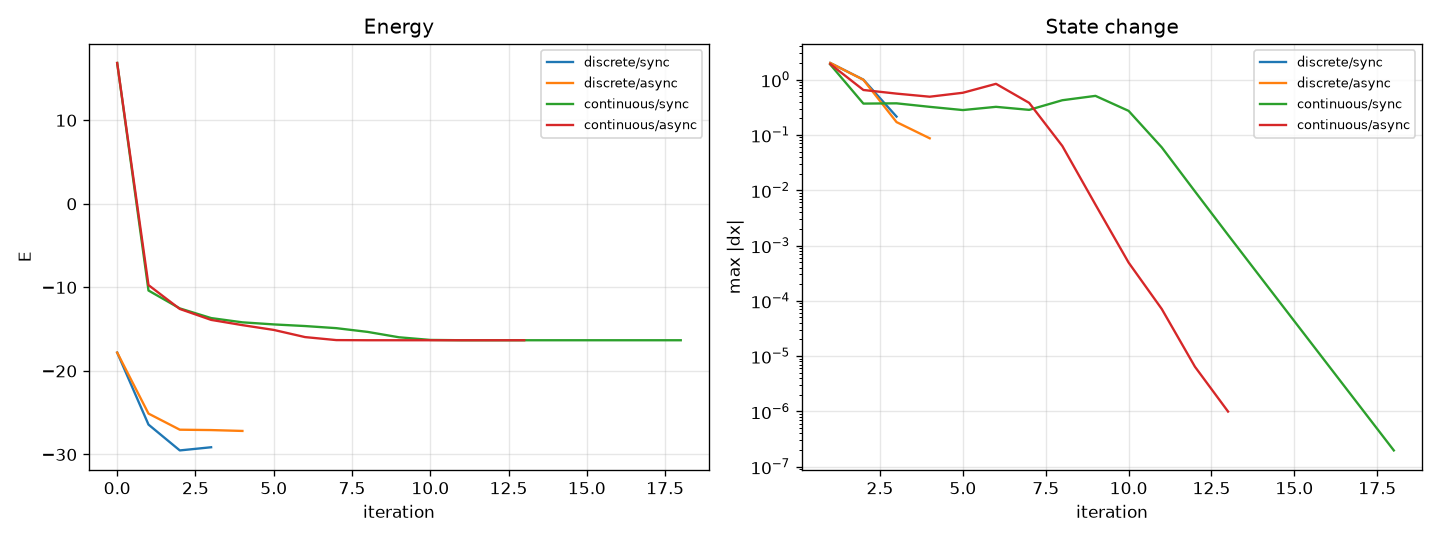
\includegraphics[width=0.95\textwidth]{energy_curves.png}
	\caption{Зависимость энергии и изменения состояния от числа итераций}
	\label{fig:energy}
\end{figure}

Энергия убывает монотонно во всех режимах, что подтверждает корректность весов и правил обновления. Дискретный режим сходится за 3--4 итерации (по стабильности знака), непрерывный~\mdash  за 13--18 итераций (по порогу $\varepsilon$). Синхронный режим сходится медленнее асинхронного, что согласуется с теорией: асинхронное обновление гарантирует спуск по энергии, синхронное~\mdash  нет.

\subsubsection{Зависимость успешности распознавания от уровня шума}

На рисунке~\ref{fig:noise} приведены семейства кривых: доля успешных распознаваний и среднее число итераций до релаксации в зависимости от уровня шума $p$ для всех четырёх режимов.

\begin{figure}[H]
	\centering
	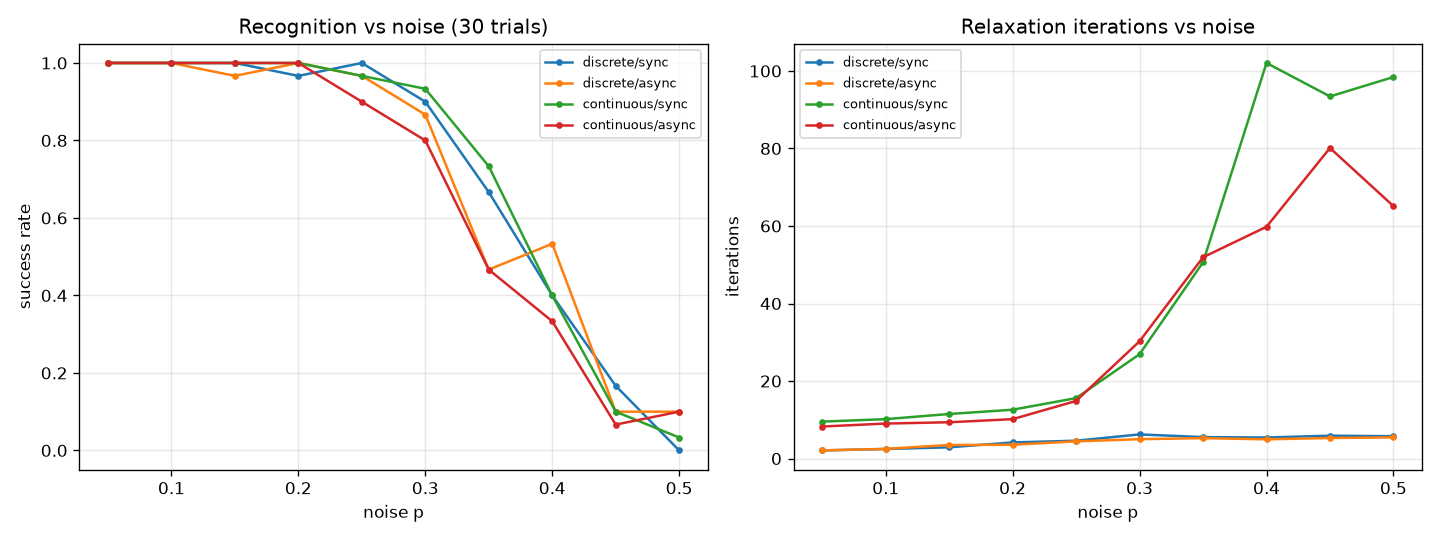
\includegraphics[width=0.95\textwidth]{noise_sweep.png}
	\caption{Успешность распознавания и число итераций в зависимости от уровня шума}
	\label{fig:noise}
\end{figure}

До уровня шума $p \le 0.2$ все режимы распознают образы практически безошибочно (успешность $\ge 0.97$). Начиная с $p \approx 0.25$--$0.3$ успешность падает, при $p = 0.5$ (полностью случайный шум) сеть деградирует до случайного угадывания. Число итераций до релаксации для непрерывного режима растёт с увеличением $p$: зашумлённый образ нужно «дотягивать» дольше. В дискретном режиме число итераций остаётся небольшим, так как критерий релаксации срабатывает, как только знаки компонент перестают меняться.

\subsubsection{Зависимость успешности от числа эталонов (ёмкость)}

На рисунке~\ref{fig:capacity} приведена зависимость успешности распознавания при $p = 0.2$ от числа запомненных эталонов $Q$ (эталоны добавляются по порядку).

\begin{figure}[H]
	\centering
	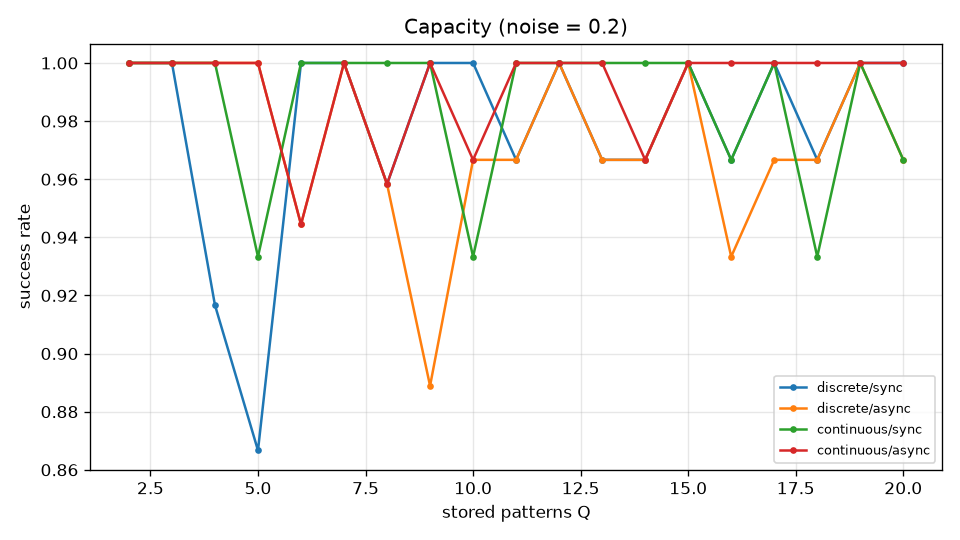
\includegraphics[width=0.8\textwidth]{capacity.png}
	\caption{Ёмкость сети: успешность в зависимости от числа эталонов}
	\label{fig:capacity}
\end{figure}

Метод проекции демонстрирует высокую ёмкость: при $Q = 20 \le n = 100$ успешность остаётся на уровне $0.93$--$1.0$ во всех режимах. Это заметное преимущество перед классическим правилом Гебба: проекционные веса гарантируют запоминание до $n$ линейно независимых образов.

\subsubsection{Визуальное распознавание}

На рисунке~\ref{fig:visual} приведена сетка результатов: первый столбец~\mdash  эталоны, последующие столбцы~\mdash  восстановление при уровнях шума $p = 0.1, 0.2, 0.3, 0.4$ (режим continuous/async).

\begin{figure}[H]
	\centering
	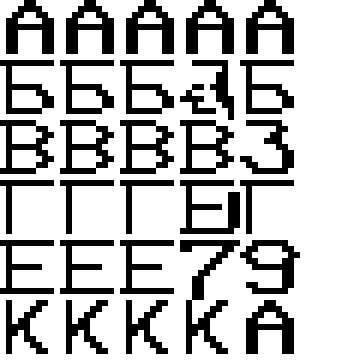
\includegraphics[width=0.95\textwidth]{visual_grid.png}
	\caption{Визуализация распознавания: эталон и восстановление при различных уровнях шума}
	\label{fig:visual}
\end{figure}

При $p \le 0.3$ восстановление практически точное, при $p = 0.4$ отдельные образы («Е», «К») ошибочно сходятся к соседним аттракторам, что иллюстрирует границы областей притяжения.

\subsection{Ответы на вопросы}

\begin{enumerate}
	\item \textbf{Что такое релаксация?} Стабилизация состояния сети: динамика прекращается, изменения состояния на последующих итерациях не превышают порог $\varepsilon$ (непрерывный режим) или знаки компонент перестают меняться (дискретный режим).
	\item \textbf{Почему синхронный режим может зацикливаться?} Одновременное обновление всех нейронов не гарантирует монотонного убывания энергии: сеть может перескакивать между двумя состояниями (цикл длины 2). Асинхронное обновление с симметричным $W$ гарантирует сходимость~\cite{haykin}.
	\item \textbf{Зачем нужен метод проекции?} Он гарантирует, что каждый эталон является точной фиксированной точкой ($W x^{(k)} = x^{(k)}$) при сохранении симметрии $W$, что обеспечивает высокую ёмкость и точность восстановления по сравнению с правилом Гебба.
	\item \textbf{Влияет ли обнуление диагонали $W$?} Да: обнуление диагонали нарушает свойство проекции $W X^{\mathsf{T}} = X^{\mathsf{T}}$, поэтому в реализации диагональ сохраняется.
	\item \textbf{Какова ёмкость сети при методе проекции?} До $n$ линейно независимых образов (при $Q \le n$ и полном ранге $X$). В эксперименте при $Q = 20$, $n = 100$ успешность $\ge 0.93$.
	\item \textbf{Роль коэффициента усиления $g$?} Масштабирует локальное поле, гарантируя насыщение функции активации ($|h_i| \ge 1$) вблизи эталонов; при $g \le 1$ модифицированная функция знака может «схлопнуть» состояние вблизи нуля из-за погрешности вычислений.
	\item \textbf{Как отличается непрерывный режим от дискретного?} В дискретном состоянии после бинаризации нейроны принимают значения из $\{-1, 1\}$ (в зашумлённом входе допускается также $0$), переходные значения выдаёт модифицированная функция знака; в непрерывном~\mdash  вещественные значения из $(-1, 1)$ через $\tanh$; критерии релаксации также различаются.
	\item \textbf{Что показывает график энергии?} Монотонное убывание $E$ подтверждает, что сеть спускается к локальному минимуму~\mdash  аттрактору, соответствующему одному из эталонов или их суперпозиции.
\end{enumerate}
